\documentclass[12pt]{article}
\usepackage[spanish]{babel}
\usepackage{natbib}
\usepackage{url}
\usepackage[utf8x]{inputenc}
\usepackage{amsmath}
\usepackage{float}
\usepackage{subfig}
\usepackage{graphicx}
\graphicspath{{images/}}
\usepackage{parskip}
\usepackage{fancyhdr}
\usepackage{vmargin}
\usepackage{mathtools}
\usepackage{amssymb} 



\title{Actividad \#6: Periodo del Péndulo }							
\author{\Large Jesùs Valenzuela Nieblas\\}											
\date{} 

\makeatletter
\let\thetitle\@title
\let\theauthor\@author
\let\thedate										
\makeatother

\pagestyle{fancy}

\lhead{\thetitle}
\cfoot{\thepage}
\rhead{}
\begin{document}

%%%%%%%%%%%%%%%%%%%%%%%%%%%%%%%%%%%%%%%%%%%%%%%%%%%%%%%%%%%%%%%%%%%%%%%%%%%%%%%%%%%%%%%%%

\begin{titlepage}
	\centering
    \vspace*{.5cm}
     
\includegraphics[scale = 0.7]{logo}\\	% University Logo
    \textsc{\Large Universidad de Sonora}\\[1.0 cm]	% University Name
	\textsc{\Large División de Ciencias Exactas y Naturales}\\[.50 cm]
  	\textsc{\Large Licenciatura en Fìsica}\\[.5 cm]
  \textsc{\large Fìsica Computacional 1}\\[1.5 cm]				% Course Name
	
	{ \huge \bfseries \thetitle}\\

    \vspace*{3 cm}
	\begin{minipage}{\textwidth}
    \centering
    \theauthor
	\end{minipage}\\[3 cm]

	\vfill
	
\end{titlepage}

%%%%%%%%%%%%%%%%%%%%%%%%%%%%%%%%%%%%%%%%%%%%%%%%%%%%%%%%%%%%%%%%%%%%%%%%%%%%%%%%%%%%%%%%%

\section{Introducciòn}
El péndulo es un sistema físico que puede oscilar bajo la acción gravitatoria u otra característica física (elasticidad, por ejemplo) y que está configurado por una masa suspendida de un punto o de un eje horizontal fijos mediante un hilo, una varilla, u otro dispositivo que sirve para medir el tiempo.
El péndulo simple es una idealización del péndulo real en un sistema aislado usando las siguientes suposiciones:
\begin{itemize}
\item La varilla o cable que sostiene la masa no se estira y siempre permanece tensa.
\item La masa es siempre puntual.
\item El movimiento u oscilación sólo se produce en dos dimensiones.
\item No hay resistencia del aire.
\item El campo gravitatorio es uniforme.
\item El soporte permanece inmóvil.
\end{itemize}

La ecuación diferencial que representa el movimiento del péndulo simple es:
\begin{equation}
\frac{d^2 \theta}{d t^2}+\frac{g}{l}\sin \theta=0
\end{equation}

Donde $g$ es la aceleración gravitacional, $l$ la longitud del péndulo y $\theta$ es el desplazamiento angular.
El movimiento es un movimiento armónico simple donde $\theta_0$ es la semi-amplitud de la oscilación (es decir, el ángulo máximo entre la varilla del péndulo y la vertical). El periodo del movimiento, el tiempo para una oscilación completa (ida y vuelta) es
\begin{equation}
T_0 = 2 \pi \sqrt {\frac {\ell} {g}} \quad \quad \quad \quad \quad 
\end{equation}
\section{Actividad}

El còdigo utilizado es el siguiente:
\begin{verbatim}
#Biblos
import numpy as np
from scipy.integrate import quad
import matplotlib.pyplot as plt

#Constantes
g=9.81 
l= 3  
n= 50
e=0.001 
T0 =np.linspace(e, (np.pi)-e, n)

#Integrales
I = [0 for i in range(n)]
E = [0 for i in range(n)]
T = [0 for i in range(n)]
To = 2.0 * np.pi*np.sqrt(l/g)

#Integrando
inte = lambda x, c : 1.0 /(np.sqrt(np.cos(x)-np.cos(c)))

for i in range(n):
    
    T1 = T0[i]
    I[i] , E [i] = quad(inte, 0, T1, args=(T1))
    T[i] = 4*np.sqrt(l/(2*g)) * I[i]
       
R=T/To

Tg= (T0*180.0)/np.pi 

#Graph
plt.plot(Tg, R, "go")
plt.grid()
plt.title("Error ")
plt.xlabel("Angulo")
plt.ylabel("Razon entre periodos")
plt.axis([0,180,1,5])
plt.show()
\end{verbatim}
\section{Gráficas}
\subsection{n=100}
\begin{figure}[H]
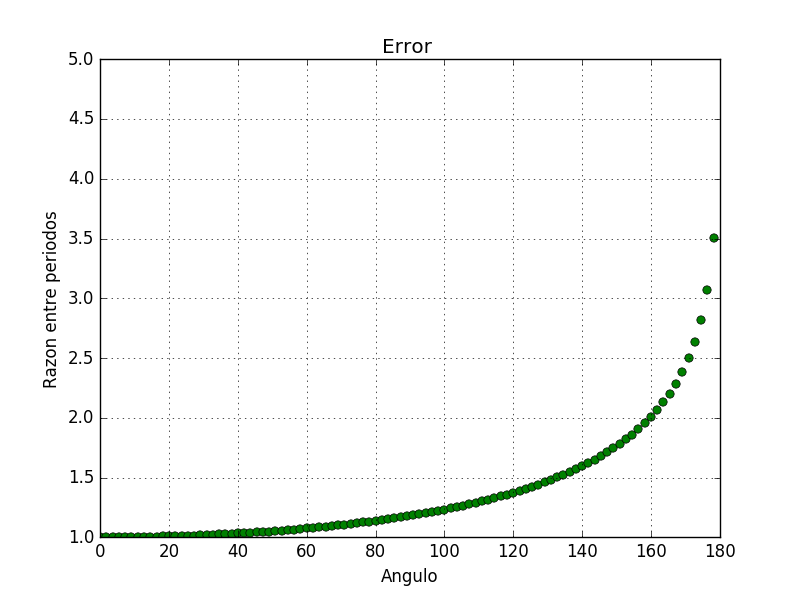
\includegraphics[scale=.6]{n100}
\end{figure}

\subsection{n=500}
\begin{figure}[H]
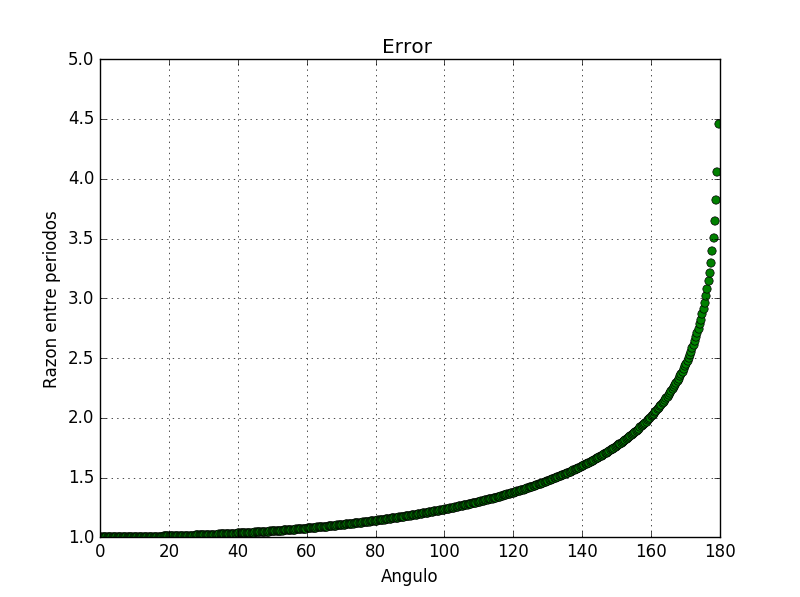
\includegraphics[scale=.6]{n500}
\end{figure}

\subsection{n =1000}
\begin{figure}[H]
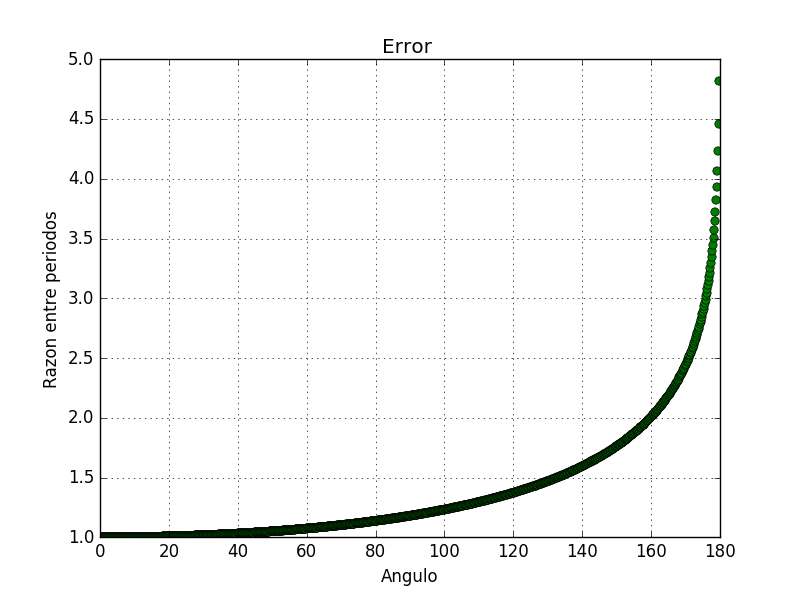
\includegraphics[scale=.6]{n1000}
\end{figure}


\end{document}
